\section{A gap in the disjoint-support relaxation}
\label{family:counterexample-section}

The disjoint-support construction includes an affine-square certificate on
every face of the cube. These certificates do not suffice for all nonnegative
quadratics, even when every square coefficient is strictly positive. The
following example gives both a geometric obstruction and an exact moment
certificate of the gap.

\begin{theorem}
\label{family:counterexample}
The quadratic
\begin{equation}
\label{family:example-polynomial}
p(x,y,z)=x^2+y^2+9z^2+6xy-12xz-12yz-x-y+9z+\tfrac14
\end{equation}
belongs to $\mathcal P_3^+$ but not to $\mathcal D_3$.
Its minimum on $C_3$ is zero, and its zero set consists of the five points
\begin{equation}
\label{family:five-zeros}
\begin{split}
a&=(\tfrac12,0,0),\qquad b=(0,\tfrac12,0),\\
c&=(1,0,\tfrac16),\qquad d=(0,1,\tfrac16),\qquad
e=(1,1,\tfrac56).
\end{split}
\end{equation}
\end{theorem}

\begin{figure}[htbp]
\centering
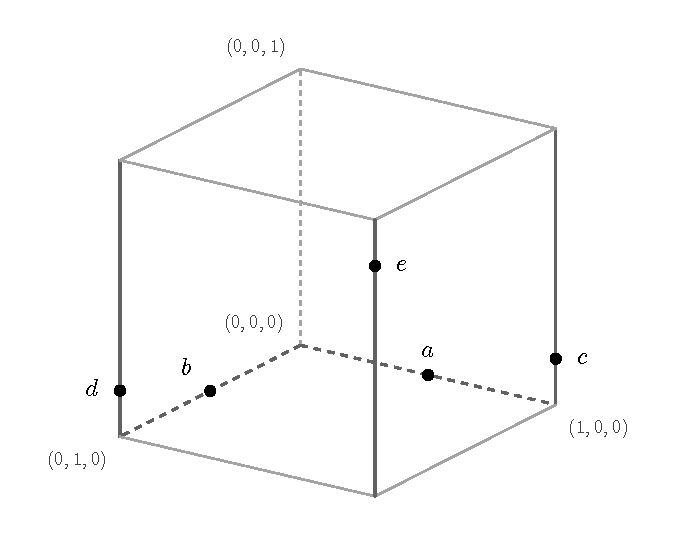
\includegraphics[width=0.60\linewidth]{figures/five-edge-zeros.pdf}
\caption{The five interior edge zeros of $p$ in \eqref{family:five-zeros}.
Darker edges contain zeros; dashed lines indicate rear cube edges.
These contacts explain the disjoint-support obstruction and determine
the exposed ray in \Cref{family:exposed}.}
\label{family:contact-figure}
\end{figure}

\begin{proof}
The polynomial identity
\begin{equation}
\label{family:example-identity}
\begin{split}
p={}&(xy+x+y-3z-\tfrac12)^2+6z(1-x)(1-y)\\
   &+3xy(1-x)+2xy(1-y)+x^2y(1-y)
\end{split}
\end{equation}
proves nonnegativity on the cube. Its square coefficients are $1,1,9$.
At a zero, the third and fourth terms imply either $xy=0$ or $x=y=1$.
If $y=0$, the second term implies $z=0$ or $x=1$; the square then gives
$a$ or $c$. The case $x=0$ gives $b$ or $d$. If $x=y=1$, the square gives
$e$. Each of these five points is indeed a zero.

Suppose that $p$ has a disjoint-support certificate. Since
$p(0,0,0)=1/4$, some individual term $w_{A,B}\ell^2$ is strictly positive
at the origin. Its weight must have $A=\varnothing$, and its affine factor
has the form
$\ell=\alpha+\beta x+\gamma y+\delta z$ with $\alpha\ne0$.
Every term in the certificate is nonnegative on the cube, so this term
vanishes at each point in \eqref{family:five-zeros}.

The weight is strictly positive at $a$ and $b$, for every possible $B$.
Thus $\beta=\gamma=-2\alpha$. The support restriction now excludes $x$
and $y$ from $B$, so $B\subseteq\{z\}$. The weight is consequently
strictly positive at $c$ and $e$. Vanishing at $c$ gives
$\delta=6\alpha$, whereas at $e$ the affine factor has value $2\alpha$.
This contradicts its required vanishing.
\end{proof}

The identity \eqref{family:example-identity} also identifies what the
disjoint construction omits. It uses a bilinear expression inside a square,
and a factor $y(1-y)$ whose two literals concern the same coordinate.
Neither is allowed in $\mathcal K_D$. The exclusion proof does not depend
on a degree truncation: in three variables all permitted generators already
have degree at most four, and all of them are included in $\mathcal K_D$.

The five zeros in \Cref{family:contact-figure} explain the obstruction.
An interior zero on an edge forces
every certificate term whose weight is positive there to vanish through
its affine factor. For a term positive at the origin, the first two zeros
force both $x$ and $y$ to occur in that factor. The remaining zeros then
impose inconsistent affine equations. This argument concerns the support
restriction, rather than the size of a chosen semidefinite block.

\begin{proposition}[Exact moment gap]
\label{family:gap}
There is a linear functional $\Lambda$ on $V$, with $\Lambda(1)=1$, such
that all $27$ disjoint localizing matrices are positive definite and
\begin{equation}
\label{family:gap-value}
\Lambda(p)=-\tfrac1{40}.
\end{equation}
Its quadratic moments also satisfy $Y_{ii}<m_i$ for all three coordinates.
In particular, $p\notin\cl(\mathcal D_3)$, and every feasible lower bound
in the certificate problem
\[
\sup\{\gamma:p-\gamma\in\mathcal D_3\}
\]
is at most $-1/40$, although $\min_{C_3}p=0$.
\end{proposition}

\begin{proof}
Use the rational moments in \cref{family:moment-table}. Their localizing
matrices and positive leading determinants are given in
\cref{family:localizing-tables}. Since
$\Lambda(w_{A,B}\ell^2)$ is the quadratic form of the corresponding
positive definite matrix, $\Lambda$ is nonnegative on $\mathcal K_D$.
Substitution in \eqref{family:example-polynomial} gives
\eqref{family:gap-value}. Continuity therefore separates $p$ from
$\cl(\mathcal D_3)$ as well as from $\mathcal D_3$.
The diagonal upper-bound slacks are
\[
m_x-Y_{xx}=m_y-Y_{yy}=\frac{649}{10000},\qquad
m_z-Y_{zz}=\frac{696}{10000}.
\]
If $p-\gamma\in\mathcal D_3$, applying $\Lambda$ gives
$-1/40-\gamma\ge0$.
\end{proof}

This gap is not confined to quadratics with zeros. The polynomial
$p+1/80$ is at least $1/80$ throughout the cube, while
$\Lambda(p+1/80)=-1/80$. Thus even strict positivity does not make these
disjoint certificates complete.

\subsection{Comparison with two recent relaxations}
\label{family:comparison-subsection}

For three positive loops, the matrices in the disjoint-support system are
exactly the $27$ matrices in equation~(17) of
\citet{Khajavirad2026SparseBoxQP}. Their orders are $4,3,2,1$, with respective
multiplicities $1,6,12,8$. Consequently,
\cref{family:gap} gives a negative answer to the three-variable exactness
question for that system. This comparison uses the displayed matrices;
it does not require a convention about the degree of the SOS certificate.

The same functional satisfies the second-order-cone strengthening of the
extended triangle inequalities in \citet{AnstreicherPuges2025ETRI}.
Let $t=\Lambda(xyz)$. For distinct indices $i,j,k$, its two types of SOC
inequalities are
\begin{equation}
\label{family:ap-soc}
t^2\le Y_{ii}Y_{jk},\qquad
(Y_{ij}+t)^2\le Y_{ii}(Y_{jj}+3Y_{jk}),
\end{equation}
together with their coordinate permutations and complements. Their
trilinear RLT inequalities are the eight nonnegative scalar localizing
blocks. \Cref{family:ap-certificate} verifies all $24$ instances of the
first inequality and all $48$ instances of the second, with strictly
positive right-hand factors. The base moment matrix is positive definite,
and the separate diagonal upper bounds hold by \cref{family:gap}.
The nonnegative scalar blocks imply the off-diagonal RLT and ordinary
triangle inequalities; the SOC inequalities imply the three extended
triangle families by Lemmas~4--5 of \citet{AnstreicherPuges2025ETRI}.

It follows that intersecting either named relaxation with $p\ge0$ is a
strict strengthening. The family introduced next gives a compact way to
enforce this inequality and its parameter variations. This conclusion
does not assert that one family block dominates either relaxation on its
own. The established exact tetrahedral description of the three-variable
hull already implies $p\ge0$ \citep{AnstreicherBurer2010}.
